\XtoCBlock{RateLimiter}
\label{block:RateLimiter}
\begin{figure}[H]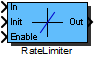
\includegraphics{RateLimiter}\end{figure} 

\begin{XtoCtabular}{Inports}
In & \tabularnewline
\hline
Init & Value which is loaded at rising flanke of enable signal\tabularnewline
\hline
Enable & Enable == 0: Deactivation of block; Out is set to In.

Enable != 0: Activation of block; Out is rate limited.

Enable 0->1: Preloading of output; Out is set to value of Init input\tabularnewline
\hline
\end{XtoCtabular}


\begin{XtoCtabular}{Outports}
Out & \tabularnewline
\hline
\end{XtoCtabular}

\begin{XtoCtabular}{Mask Parameters}
Tr & Rising time in seconds. Slew rate will be 1/Tr\tabularnewline
\hline
Tf & Falling time in seconds. Slew rate will be 1/Tf\tabularnewline
\hline
ts\_fact & Multiplication factor of base sampling time (in integer format)\tabularnewline
\hline
\end{XtoCtabular}

\subsubsection*{Description:}
Limitation of rising and falling rate.

    Function of Enable:

        0:       rate limiting disabled, signal is passed through

        1:       rate limiting enabled, signal is rate limited

        0->1: preload of output with value from init input

% include optional documentation file
\InputIfFileExists{\XcHomePath/Library/General/Doc/RateLimiter_Info.tex}{\vspace{1ex}}{}

\subsubsection*{Implementations:}
\begin{tabular}{l l}
\textbf{FiP8} & 8 Bit Fixed Point Implementation\tabularnewline
\textbf{FiP16} & 16 Bit Fixed Point Implementation\tabularnewline
\textbf{FiP32} & 32 Bit Fixed Point Implementation\tabularnewline
\textbf{Float32} & 32 Bit Floating Point Implementation\tabularnewline
\textbf{Float64} & 64 Bit Floating Point Implementation\tabularnewline
\end{tabular}

\XtoCImplementation{FiP8}
\index{Block ID!96}
\nopagebreak[0]
% Implementation details
\begin{tabular}{l l}
\textbf{Name} & FiP8 \tabularnewline
\textbf{ID} & 96 \tabularnewline
\textbf{Revision} & 1.0 \tabularnewline
\textbf{C filename} & RateLimiter\_FiP8.c \tabularnewline
\textbf{H filename} & RateLimiter\_FiP8.h \tabularnewline
\end{tabular}
\vspace{1ex}

8 Bit Fixed Point Implementation

\begin{XtoCtabular}{Controller Parameters}
RateUp & Rising time parameter\tabularnewline
\hline
RateDown & Falling time parameter\tabularnewline
\hline
out\_old & Output value from last cycle in int16 format\tabularnewline
\hline
enable\_old & Enable value from last cycle\tabularnewline
\hline
\end{XtoCtabular}

% Implementation data structure
\XtoCDataStruct{Data Structure:}
\begin{lstlisting}
typedef struct {
     uint16        ID;
     int8          *In;
     int8          *Init;
     int8          *Enable;
     int8          Out;
     int16         RateUp;
     int16         RateDown;
     int16         out_old;
     int8          enable_old;
} RATELIMITER_FIP8;
\end{lstlisting}

\ifdefined \AddTestReports
\InputIfFileExists{\XcHomePath/Library/General/Doc/Test_RateLimiter_FiP8.tex}{}{}
\fi
\XtoCImplementation{FiP16}
\index{Block ID!97}
\nopagebreak[0]
% Implementation details
\begin{tabular}{l l}
\textbf{Name} & FiP16 \tabularnewline
\textbf{ID} & 97 \tabularnewline
\textbf{Revision} & 1.0 \tabularnewline
\textbf{C filename} & RateLimiter\_FiP16.c \tabularnewline
\textbf{H filename} & RateLimiter\_FiP16.h \tabularnewline
\end{tabular}
\vspace{1ex}

16 Bit Fixed Point Implementation

\begin{XtoCtabular}{Controller Parameters}
RateUp & Rising time parameter\tabularnewline
\hline
RateDown & Falling time parameter\tabularnewline
\hline
out\_old & Output value from last cycle in int32 format\tabularnewline
\hline
enable\_old & Enable value from last cycle\tabularnewline
\hline
\end{XtoCtabular}

% Implementation data structure
\XtoCDataStruct{Data Structure:}
\begin{lstlisting}
typedef struct {
     uint16        ID;
     int16         *In;
     int16         *Init;
     int8          *Enable;
     int16         Out;
     int32         RateUp;
     int32         RateDown;
     int32         out_old;
     int8          enable_old;
} RATELIMITER_FIP16;
\end{lstlisting}

\ifdefined \AddTestReports
\InputIfFileExists{\XcHomePath/Library/General/Doc/Test_RateLimiter_FiP16.tex}{}{}
\fi
\XtoCImplementation{FiP32}
\index{Block ID!98}
\nopagebreak[0]
% Implementation details
\begin{tabular}{l l}
\textbf{Name} & FiP32 \tabularnewline
\textbf{ID} & 98 \tabularnewline
\textbf{Revision} & 1.0 \tabularnewline
\textbf{C filename} & RateLimiter\_FiP32.c \tabularnewline
\textbf{H filename} & RateLimiter\_FiP32.h \tabularnewline
\end{tabular}
\vspace{1ex}

32 Bit Fixed Point Implementation

\begin{XtoCtabular}{Controller Parameters}
RateUp & Rising time parameter\tabularnewline
\hline
RateDown & Falling time parameter\tabularnewline
\hline
enable\_old & Enable value from last cycle\tabularnewline
\hline
\end{XtoCtabular}

% Implementation data structure
\XtoCDataStruct{Data Structure:}
\begin{lstlisting}
typedef struct {
     uint16        ID;
     int32         *In;
     int32         *Init;
     int8          *Enable;
     int32         Out;
     int32         RateUp;
     int32         RateDown;
     int8          enable_old;
} RATELIMITER_FIP32;
\end{lstlisting}

\ifdefined \AddTestReports
\InputIfFileExists{\XcHomePath/Library/General/Doc/Test_RateLimiter_FiP32.tex}{}{}
\fi
\XtoCImplementation{Float32}
\index{Block ID!99}
\nopagebreak[0]
% Implementation details
\begin{tabular}{l l}
\textbf{Name} & Float32 \tabularnewline
\textbf{ID} & 99 \tabularnewline
\textbf{Revision} & 0.1 \tabularnewline
\textbf{C filename} & RateLimiter\_Float32.c \tabularnewline
\textbf{H filename} & RateLimiter\_Float32.h \tabularnewline
\end{tabular}
\vspace{1ex}

32 Bit Floating Point Implementation

\begin{XtoCtabular}{Controller Parameters}
RateUp & Rising time parameter\tabularnewline
\hline
RateDown & Falling time parameter\tabularnewline
\hline
enable\_old & Enable value from last cycle\tabularnewline
\hline
\end{XtoCtabular}

% Implementation data structure
\XtoCDataStruct{Data Structure:}
\begin{lstlisting}
typedef struct {
     uint16        ID;
     float32       *In;
     float32       *Init;
     int8          *Enable;
     float32       Out;
     float32       RateUp;
     float32       RateDown;
     int8          enable_old;
} RATELIMITER_FLOAT32;
\end{lstlisting}

\ifdefined \AddTestReports
\InputIfFileExists{\XcHomePath/Library/General/Doc/Test_RateLimiter_Float32.tex}{}{}
\fi
\XtoCImplementation{Float64}
\index{Block ID!100}
\nopagebreak[0]
% Implementation details
\begin{tabular}{l l}
\textbf{Name} & Float64 \tabularnewline
\textbf{ID} & 100 \tabularnewline
\textbf{Revision} & 0.1 \tabularnewline
\textbf{C filename} & RateLimiter\_Float64.c \tabularnewline
\textbf{H filename} & RateLimiter\_Float64.h \tabularnewline
\end{tabular}
\vspace{1ex}

64 Bit Floating Point Implementation

\begin{XtoCtabular}{Controller Parameters}
RateUp & Rising time parameter\tabularnewline
\hline
RateDown & Falling time parameter\tabularnewline
\hline
enable\_old & Enable value from last cycle\tabularnewline
\hline
\end{XtoCtabular}

% Implementation data structure
\XtoCDataStruct{Data Structure:}
\begin{lstlisting}
typedef struct {
     uint16        ID;
     float64       *In;
     float64       *Init;
     int8          *Enable;
     float64       Out;
     float64       RateUp;
     float64       RateDown;
     int8          enable_old;
} RATELIMITER_FLOAT64;
\end{lstlisting}

\ifdefined \AddTestReports
\InputIfFileExists{\XcHomePath/Library/General/Doc/Test_RateLimiter_Float64.tex}{}{}
\fi
